\subsection {Sprint 1}

A \textit{Sprint} 1 pode ser caracterizada pelo início dos trabalhos, onde houve foco nos três requisitos que eram centrais na proposta de melhoria do componente:

\begin{itemize}
	\item \textbf{Requisito 1 da Sprint 1}: Diminuir o tempo de renderização da página de visualização do texto participativo;
	\item \textbf{Requisito 2 da Sprint 1}: Possibilitar a criação de textos participativos através de um editor de textos próprio do Brasil Participativo, contando com o uso do comando copiar e colar, trazendo texto de fontes como o Microsoft Word e Google Docs;
	\item \textbf{Requisito 3 da Sprint 1}: Refatoração da página de visualização do rascunho (edição de parágrafos), trazendo-a para o mesmo padrão de \textit{design} que a tela de visualização.
\end{itemize}

Em acordo com o time de produto  do Lab Livre, o objetivo central era fazer um \textit{Minimum Viable Product} (MVP) para servir como uma espécie de prova de conceito, onde analisariam os resultados obtidos para eventualmente tomar uma decisão de manter ou não a mesma estratégia, a fim satisfazer as necessidades levantadas pelos \textit{stakeholders}. As próximas seções revelam detalhes da abordagem utilizada no desenvolvimento de cada requisito que foi listado acima.

\subsubsection {Requisito 1 da Sprint 1}

Aplicações \textit{Ruby on Rails} possuem um sistema de \textit{logs} que permitem que o desenvolvedor obtenha informações da execução de vários tipos e em vários níveis de detalhamento, sendo eles:

\begin{itemize}
	\item \textit{debug};
	\item \textit{info};
	\item \textit{warn};
	\item \textit{error};
	\item \textit{fatal};
	\item \textit{unknown}.
\end{itemize}

Por padrão, aplicações \textit{Rails} executadas em modo de desenvolvimento terão seu nível de \textit{log} como \textit{debug}, e quando executada em modo produtivo será \textit{info} \cite{debugging-rails-applications}.

Na condução dessa análise, o Brasil Participativo foi executado em modo desenvolvimento com nível de \textit{logs} como \textit{debug}. Com esse nível de informações, é possível visualizar na saída padrão do Puma quais consultas SQL estão sendo executadas, quais \textit{views} estão sendo renderizadas pelo \textit{Rails} durante a requisição e acessos ao ActiveStorage. Alguns desses registros são acompanhados pelo tempo gasto na execução e em alguns casos a quantidade de alocações também é informada.

Para realizar o primeiro diagnóstico, foi criado um texto participativo com em torno de 600 parágrafos, em seguida foi acessada a página de visualização do texto. A Figura \ref{fig:analise-log-600-paragrafos} mostra os \textit{logs} apresentados pela aplicação no processamento da requisição. Nota-se que a maior parte do tempo foi utilizado na renderização da \textit{views} e suas \textit{partials}, correspondendo a 96,7\% do tempo total gasto para processar a requisição.

\begin{figure}[htbp]
  \centering
  \caption{Captura de tela dos \textit{logs} apresentados pelo \textit{Rails}}
  \label{fig:analise-log-600-paragrafos}
  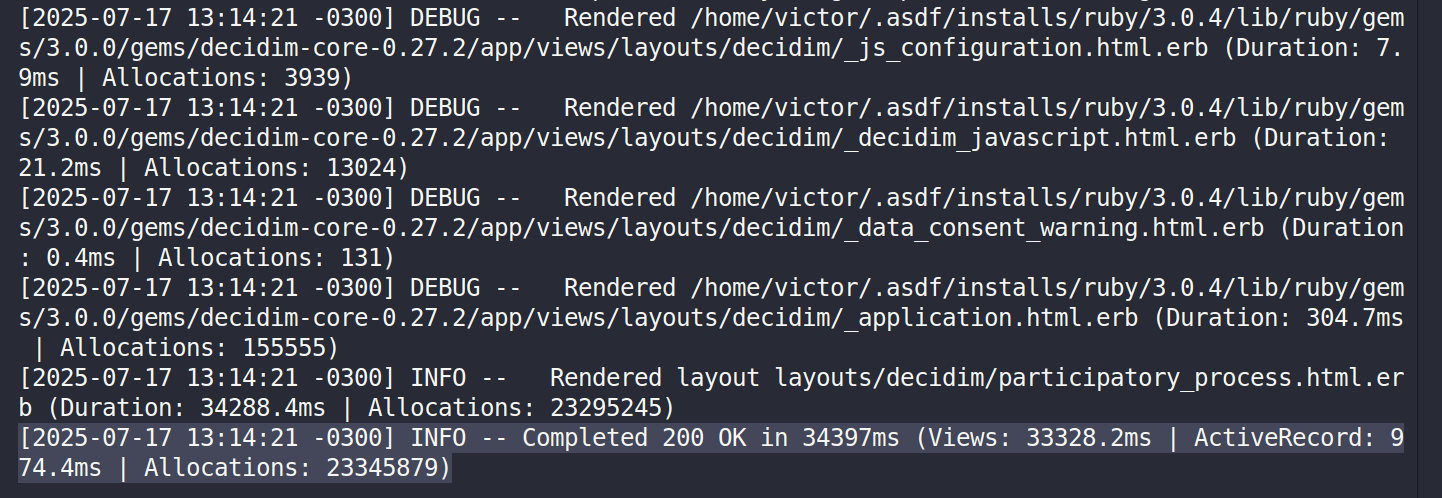
\includegraphics[width=\textwidth]{figuras/analise-log-600-paragrafos.png}
  \fonte{Próprio autor}
\end{figure}

O Decidim possui um mecanismo de representação para UI chamado de \textit{View Models}, também conhecido como \textit{cells}, em português células. Uma célula é um objeto que representa fragmentos da UI, podendo conter desde uma página inteira até um container de comentário ou imagem, por exemplo \cite{decidim-view-models-aka-cells}.

A célula \texttt{ParticipatoryTextProposalCell} é usada para realizar a renderização dos parágrafos do texto participativo. Nessa célula, são utilizados dois arquivos de \textit{view}: \texttt{show.erb} e \texttt{buttons.erb}. Para realizar a renderização de cada parágrafo, o Decidim fará duas chamadas de renderização de \textit{partials}, uma para o arquivo \texttt{show.erb} e outra para o arquivo \texttt{buttons.erb}, que é referenciado pelo arquivo \texttt{show.erb}. Esse comportamento pode ser percebido através do recorte das mensagens de \textit{log} no processamento da requisição, que é mostrado na Figura \ref{fig:logs-partials-show-buttons-evidencia}.

\begin{figure}[htbp]
  \centering
  \caption{Captura de tela dos \textit{logs} evidenciando a utilização de \textit{partials}}
  \label{fig:logs-partials-show-buttons-evidencia}
  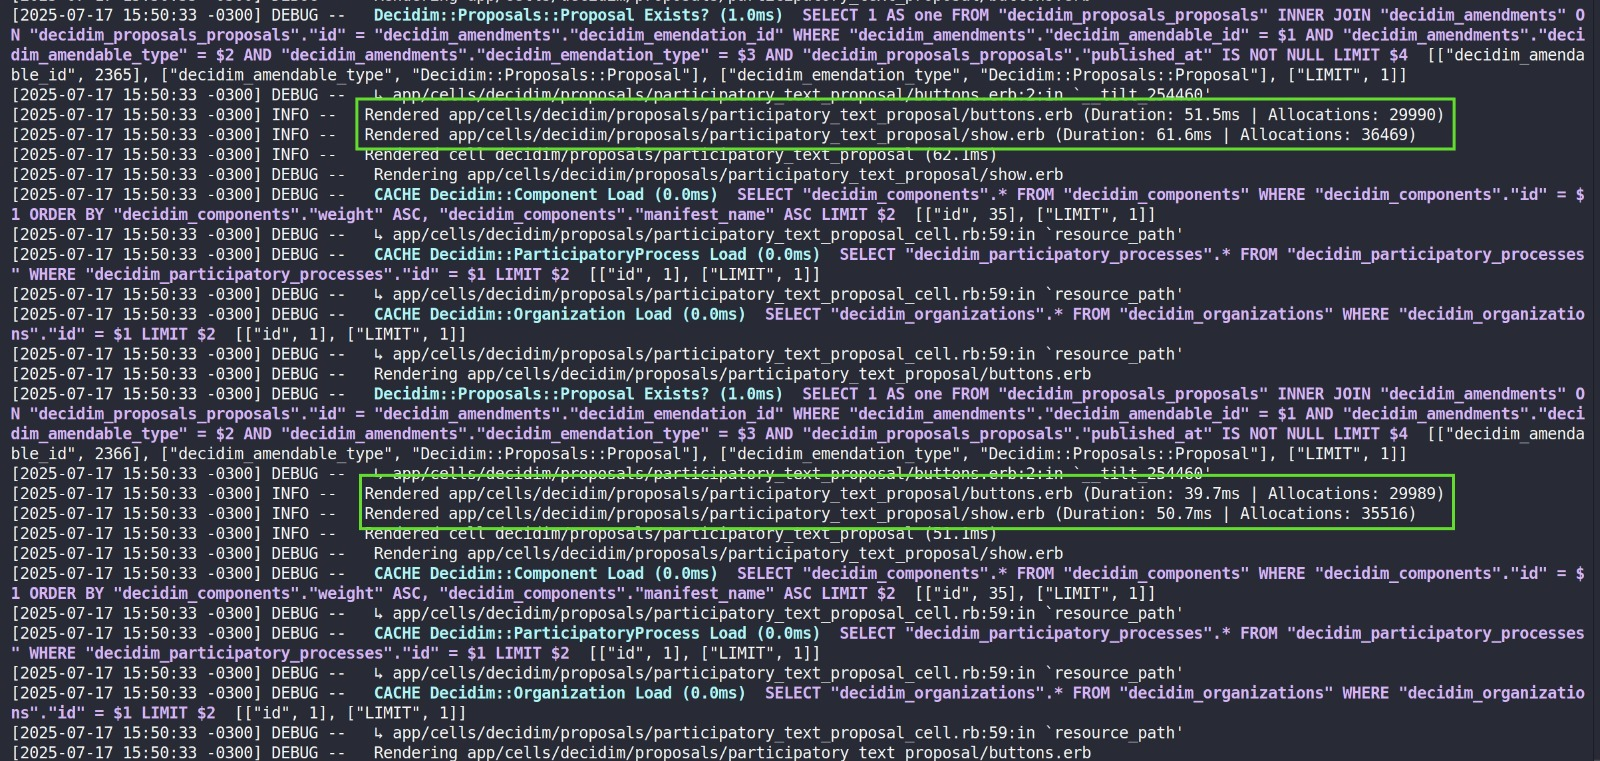
\includegraphics[width=\textwidth]{figuras/logs-partials-show-buttons-evidencia.jpeg}
  \fonte{Próprio autor}
\end{figure}

No repositório oficial do \textit{Ruby on Rails} existe uma \textit{issue} que relata problemas de desempenho com o uso de \textit{partials} em contextos onde há aninhamento, destacando que a renderização de HTML planos acontece com maior agilidade. A \textit{issue} pode ser acessada em \url{https://github.com/rails/rails/issues/41452}.

Dessa forma, a primeira tentativa de ajustes realizada foi a substituição do uso das células na renderização de textos participativos pela renderização \textit{inline} do conteúdo do parágrafo diretamente no arquivo principal da \textit{view}:

\begin{table}[h]
	\begin{tabular}{c}
		\texttt{decidim/proposals/proposals/participatory\_texts/participatory\_text.html.erb}
	\end{tabular}
\end{table}

Após realizar a substituição, foi observado novamente os \textit{logs} do processamento da requisição de renderização da página do texto participativo. O tempo de processamento total da requisição diminuiu de 34.397 milissegundos para 1.139 milissegundos, representando uma redução de 3.019,9\%, e que foi considerada como suficiente para o requisito. Uma captura de tela dos \textit{logs} é exibida na Figura \ref{fig:analise-log-apos-substituicao-celulas}.

Para elucidar a alteração, dado o enfoque deste trabalho na otimização de desempenho, o código fonte será demonstrado em capturas de tela. Contudo, as alterações estão disponíveis no repositório oficial do Brasil Participativo no \textit{Merge Request} em \url{https://gitlab.com/lappis-unb/decidimbr/decidim-govbr/-/merge\_requests/560}.

A versão anterior à modificação pode ser vista na Figura \ref{fig:versao-com-celula}, e a versão ajustada para melhora de desempenho pode ser vista na Figura \ref{fig:versao-inline}.

\begin{figure}[htbp]
  \centering
  \caption{Captura de tela dos \textit{logs} após substituição das células}
  \label{fig:analise-log-apos-substituicao-celulas}
  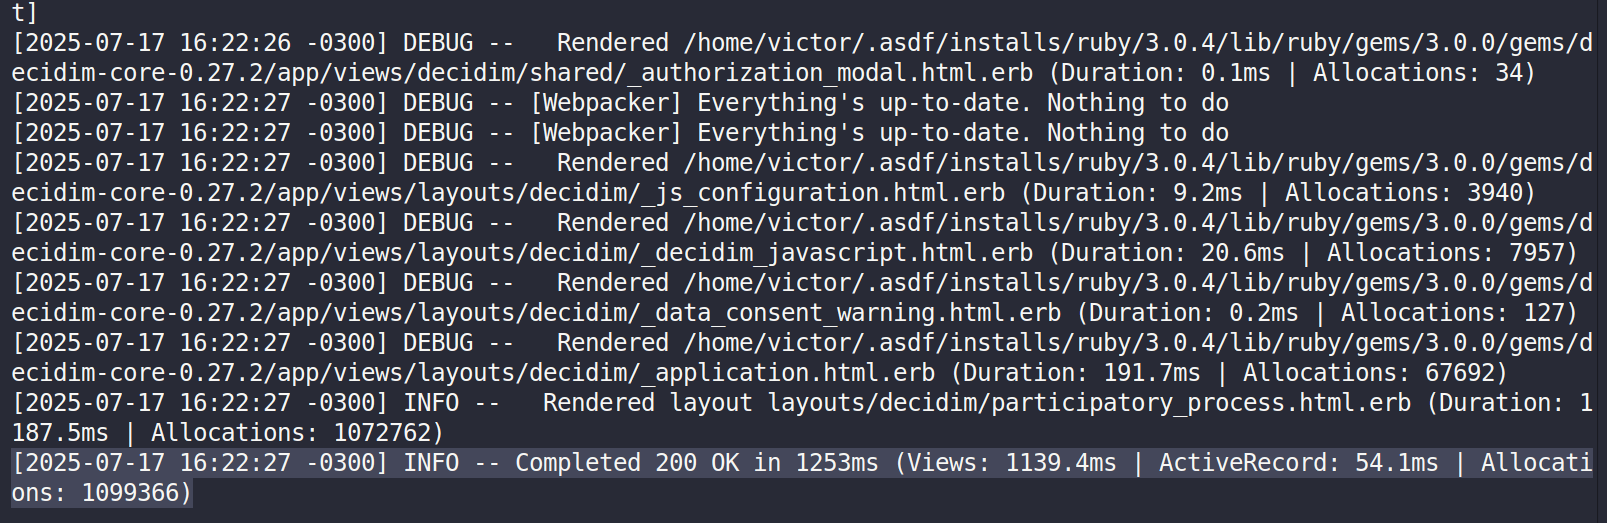
\includegraphics[width=\textwidth]{figuras/analise-log-apos-substituicao-celulas.png}
  \fonte{Próprio autor}
\end{figure}

\begin{figure}[htbp]
  \centering
  \caption{Código fonte da \textit{view} antes da substituição da célula}
  \label{fig:versao-com-celula}
  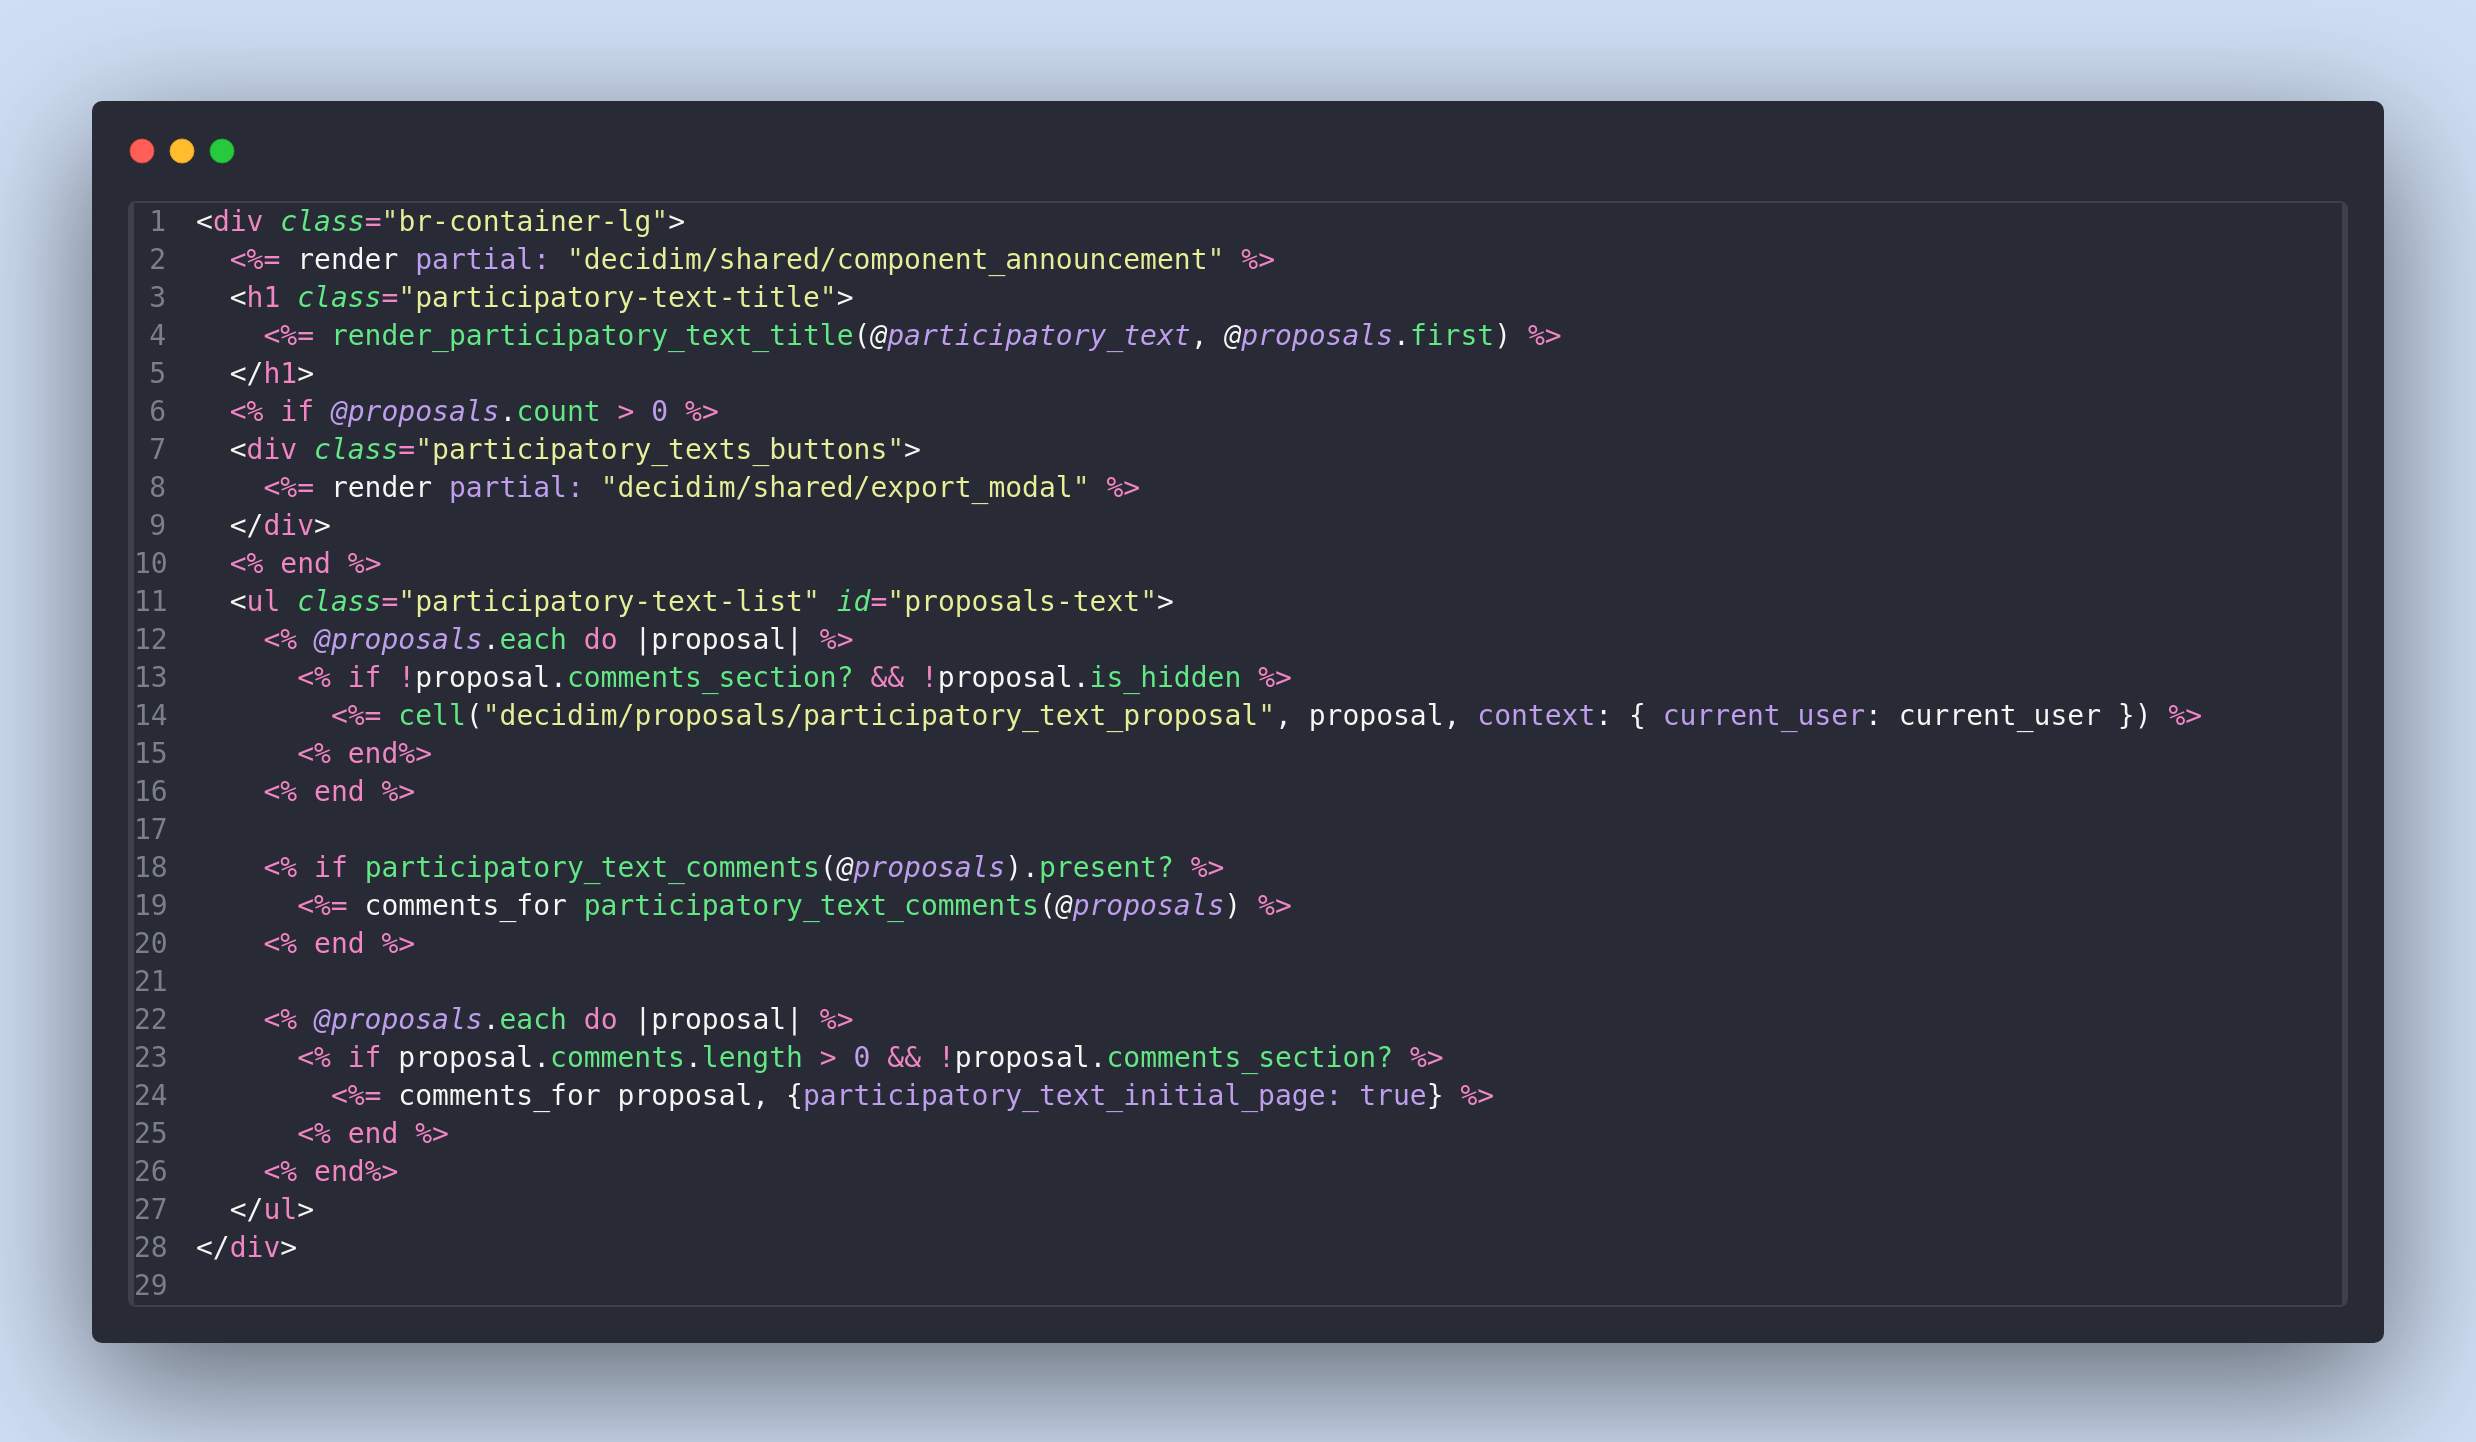
\includegraphics[width=\textwidth]{figuras/versao-celulas-1.png}
  \fonte{Próprio autor}
\end{figure}

\begin{figure}[htbp]
  \centering
  \caption{Código fonte da \textit{view} ajustado para desempenho}
  \label{fig:versao-inline}
  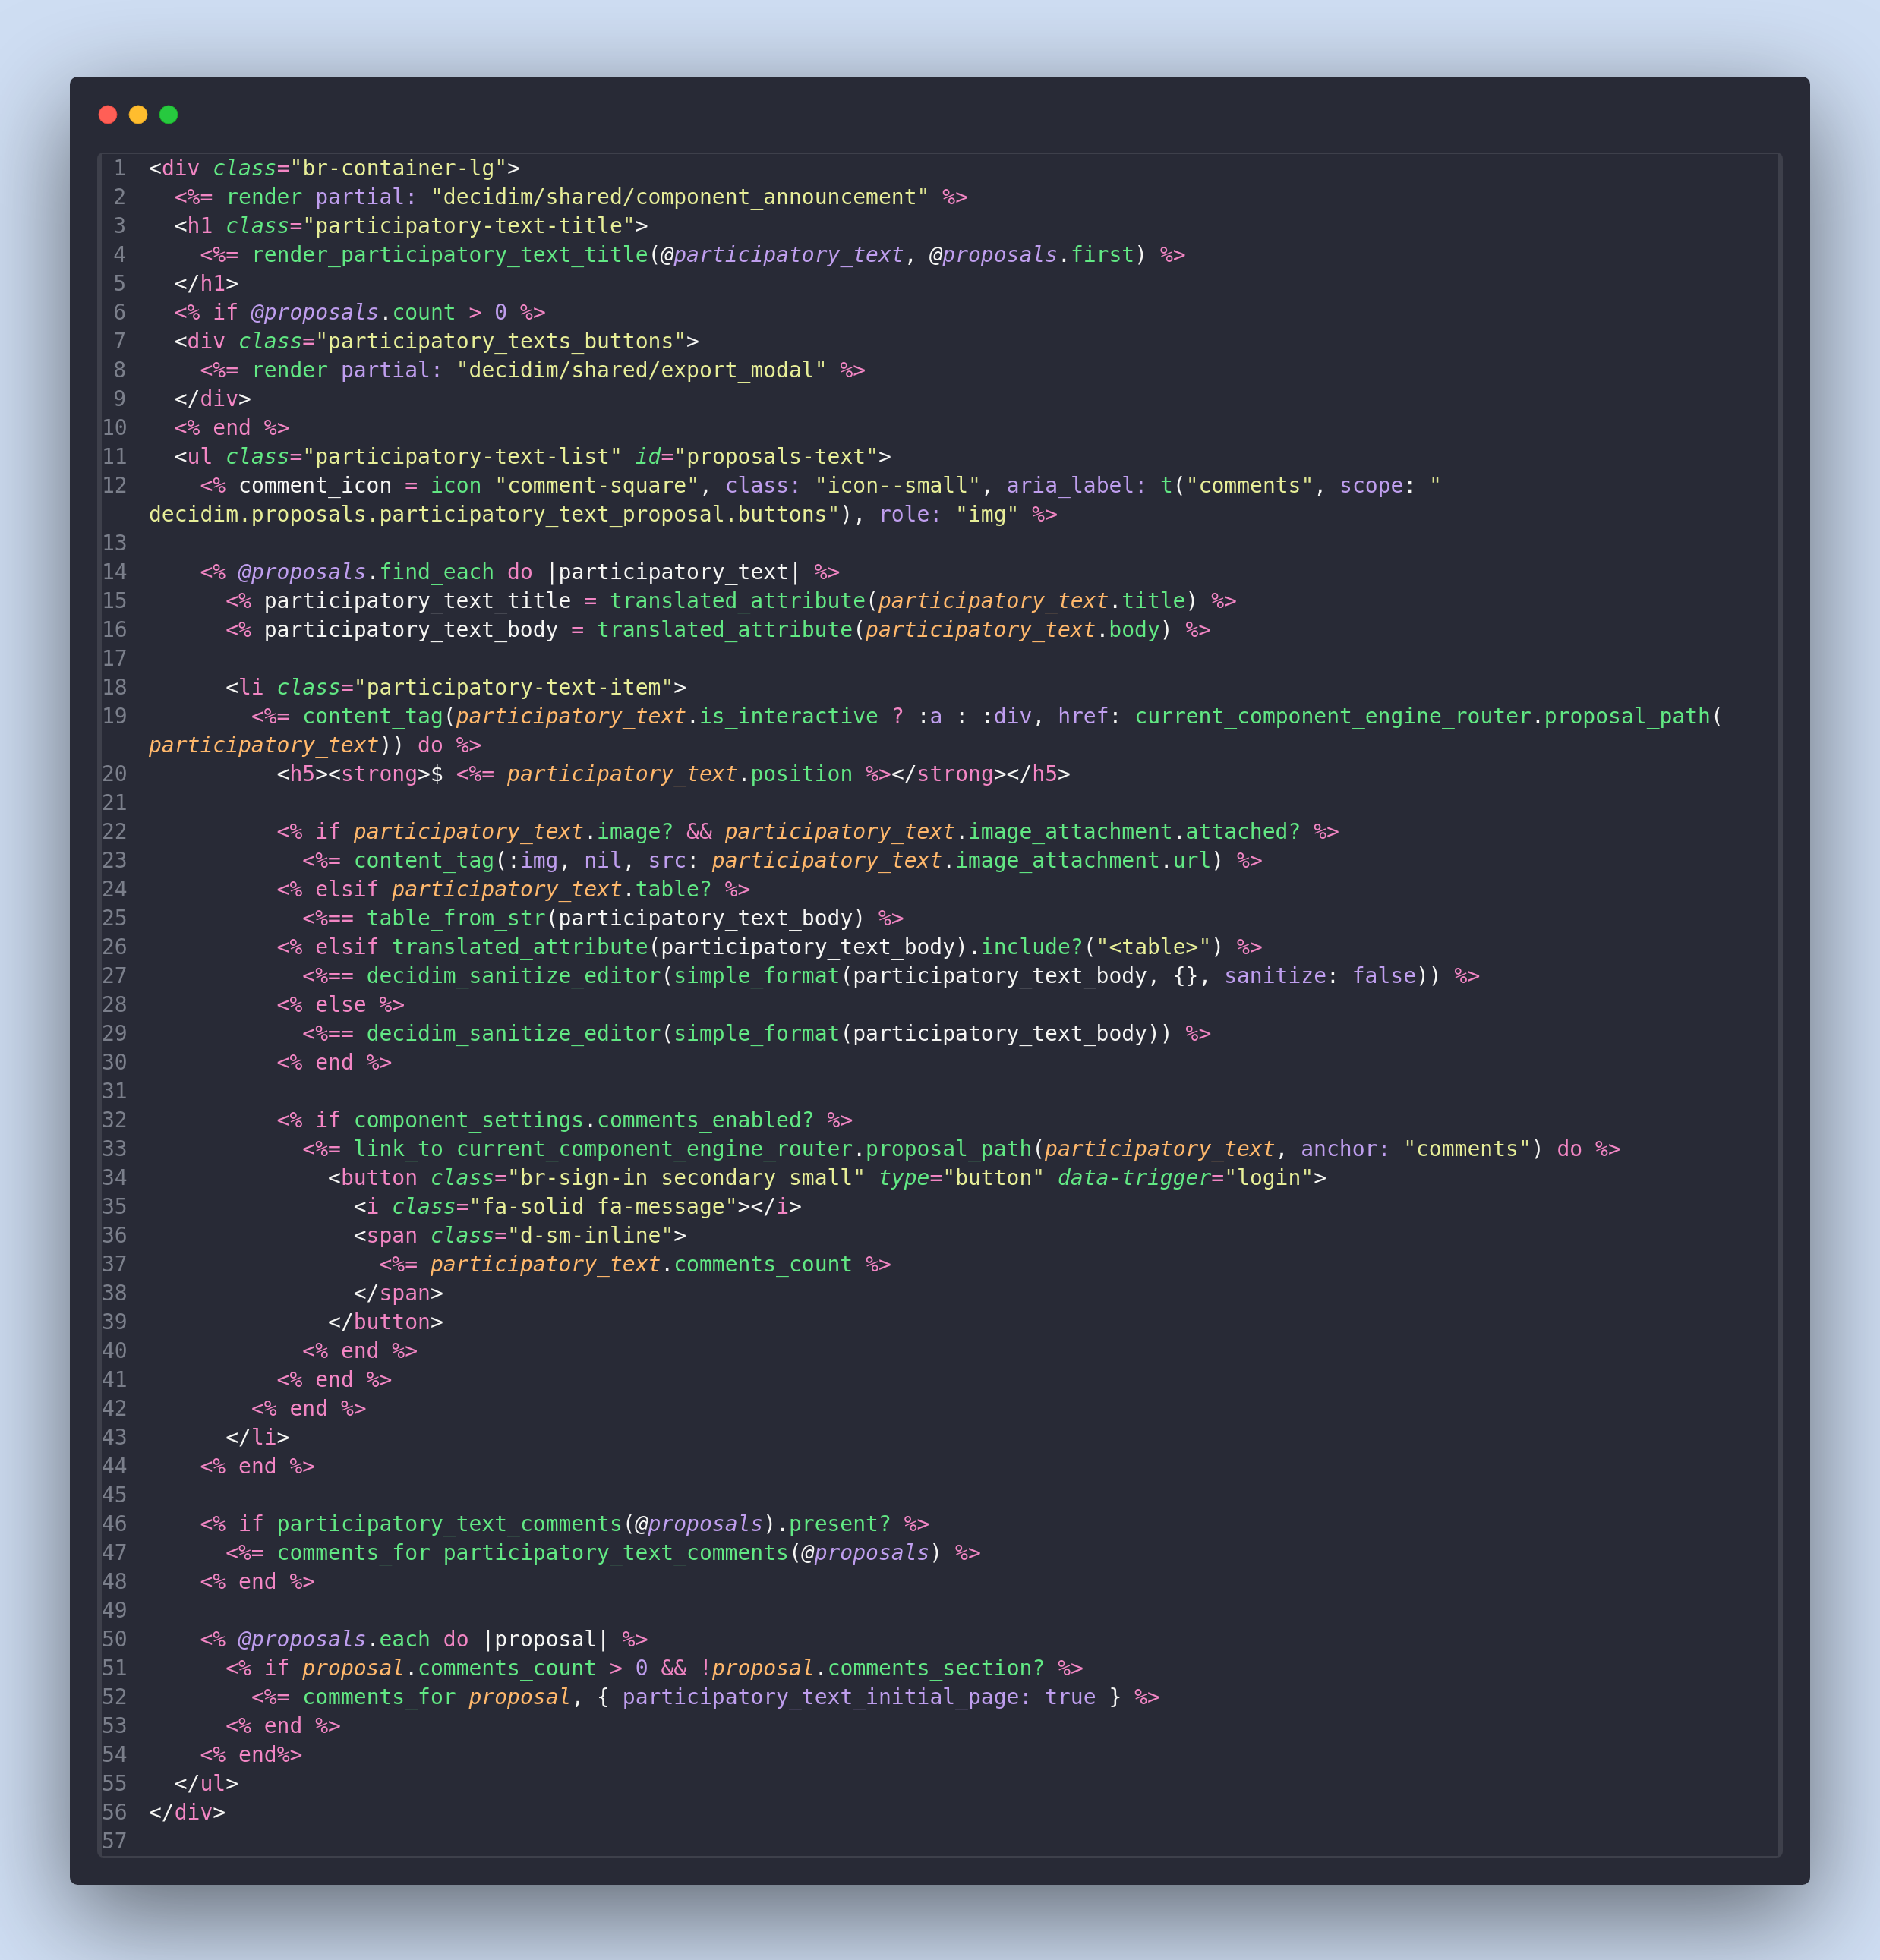
\includegraphics[width=\textwidth]{figuras/versao-inline-1.png}
  \fonte{Próprio autor}
\end{figure}

\subsubsection {Requisito 2 da Sprint 1}

Para cumprir com o segundo requisito, foi adicionado no Brasil Participativo, o editor de textos Trix que é do tipo WYSIWYG. O Trix é um editor de textos pensado para o uso de envio de mensagens, escrita de comentários, artigos e listas. Ele foi criado pela 37signals e está presente em algumas aplicações modernas, como por exemplo o Basecamp, que é uma ferramenta de gestão de projetos também da 37signals. A escolha desse editor de texto se deu pela sua facilidade de integrar com uma aplicação \textit{Rails}, e sua arquitetura baseada em eventos; permitindo com que customizações sejam feitas com pouco código.

Um requisito implícito no requisito 2 era a necessidade de inserir imagens no texto. Por padrão, o Trix posiciona a imagem no texto como um documento "pendente", portanto, é necessário que a aplicação guarde a imagem remotamente e forneça ao Trix um \textit{link} permanente.

Para realizar isso, a \textit{controller} \texttt{Decidim::Govbr::AttachmentsController} foi criada no Brasil Participativo. Esta \textit{controller} possui como papel: receber um arquivo, salvá-lo no \texttt{storage} da aplicação e devolver a URL permanente para aquele arquivo em uma resposta no formato JSON. Essa \textit{controller} ficou expôs a \textit{action} \texttt{create} na rota \texttt{/attachments}. A \textit{action} verifica antes de processar a requisição se o emissor é um usuário logado. O código da \textit{controller} é exibido na Figura \ref{fig:attachments-controller}.

\begin{figure}[htbp]
  \centering
  \caption{Código fonte da \textit{controller} \texttt{Attachments}}
  \label{fig:attachments-controller}
  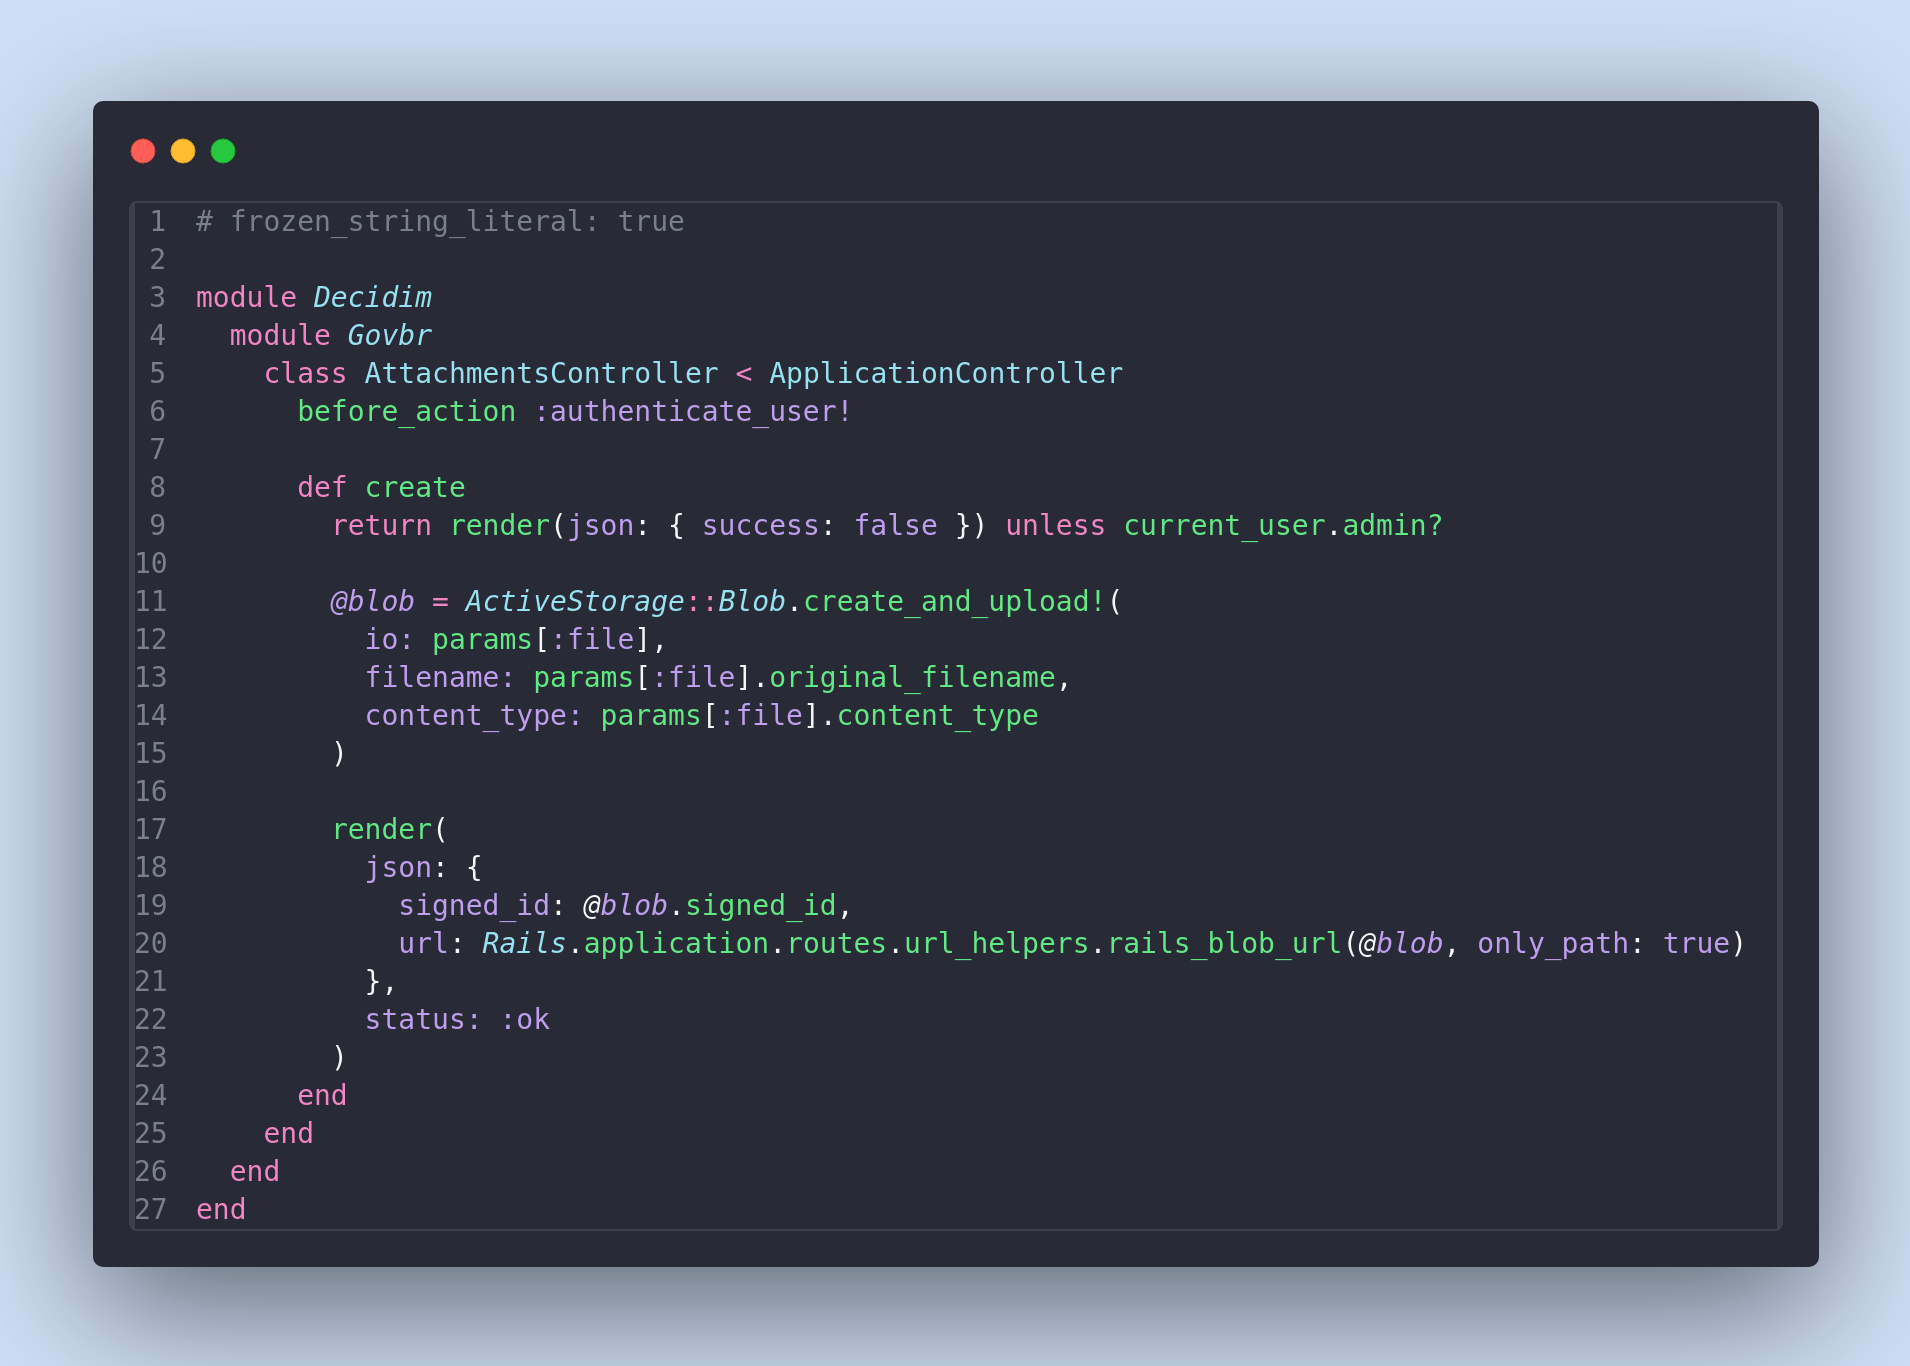
\includegraphics[width=\textwidth]{figuras/attachments-controller.png}
  \fonte{Próprio autor}
\end{figure}

Outro desafio relacionado à inserção do texto através do comando copiar e colar é separar corretamente cada parágrafo de texto. O input do usuário, apesar de parecer apenas texto, na verdade é enviado para o \textit{backend} como uma \texttt{string} HTML, como por exemplo:

\texttt{
<h1>Título do Texto</h1>
<div>
  Parágrafo! Aqui vem o conteúdo do parágrafo do usuário.<br>
  Aqui é outro parágrafo.<br>
</div>
}

Para processar o \textit{input} HTML e transformar em uma estrutura mais flexível de se trabalhar, foi adotada a \textit{gem} Nokogiri. Com o uso do Nokogiri, o texto HTML é transformado em uma estrutura de dados semelhante a uma árvore, onde cada \textit{tag} HTML se torna um nó, com seus elementos filhos, que podem ser outras \textit{tags} ou texto puro, estando disponíveis no atributo \texttt{\#children}.

A fim de separar o texto, depois de realizar o \textit{parsing} do HTML, cada elemento (\textit{tag}) de primeiro nível era considerado um parágrafo. Entretanto, quando o usuário digita um parágrafo e logo em seguida uma quebra de linha para digitar outro parágrafo, o Trix envolvia ambos os parágrafos em uma única \textit{tag} \texttt{<div>}, separando os parágrafos por quebra linha com a \textit{tag} \texttt{<br>}. Para contornar isso, foi adicionada uma verificação no nó, e caso este seja um elemento do tipo \texttt{<div>}, ele não será utilizado como um parágrafo, mas sim os seus elementos filhos diretos, desde que não seja uma \textit{tag} \texttt{<br>}. O código de divisão pode ser conferido na Figura \ref{fig:trix-paragraph-split}.

\begin{figure}[htbp]
  \centering
  \caption{Método para realizar a divisão dos parágrafos do input do usuário}
  \label{fig:trix-paragraph-split}
  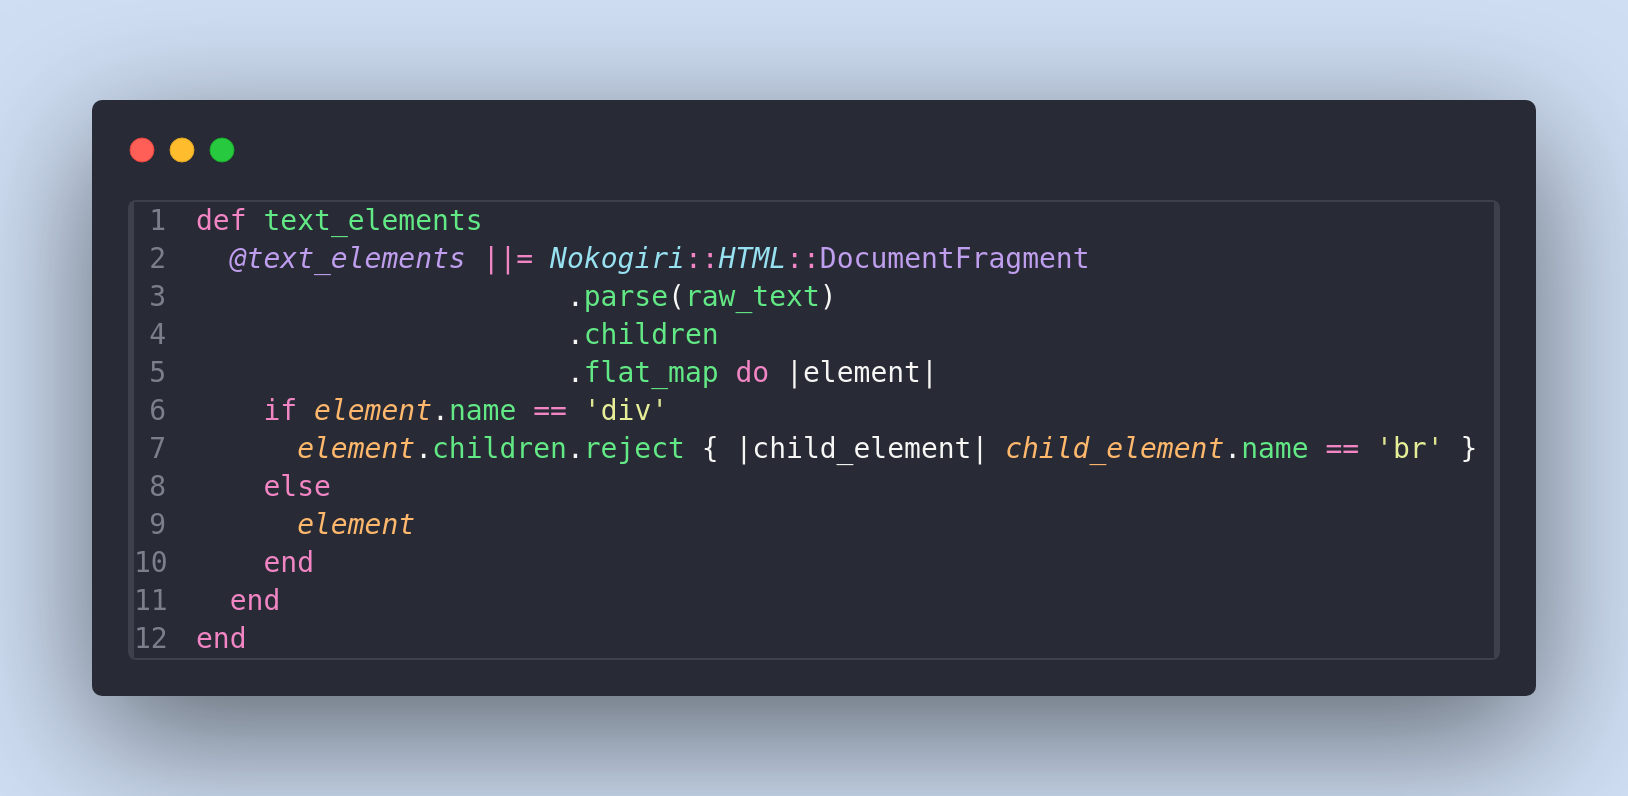
\includegraphics[width=\textwidth]{figuras/trix-paragraph-split.png}
  \fonte{Próprio autor}
\end{figure}

Depois de resolvido o problema de divisão dos parágrafos, havia a gestão das imagens presentes no texto. Dado que cada imagem é enviada para o \texttt{storage} do \textit{Rails} já no momento em que o usuário está digitando o conteúdo do texto no \textit{frontend}, era necessário de alguma maneira saber vincular cada imagem a cada parágrafo.

Um parágrafo na ferramenta de textos participativos é um objeto do tipo \texttt{Proposal}, que também é utilizado para representar propostas na plataforma. No Brasil Participativo, foi feito pela equipe de desenvolvimento do Lab Livre uma customização que permite que cada proposta tenha relacionamento com nenhum ou vários arquivos. Sendo assim, uma das etapas de pré-processamento do \textit{input} é descobrir as imagens que já estão no \texttt{storage} do \textit{Rails} e vinculá-las a cada proposta (parágrafo).

A primeira etapa é feita através da extração do atributo \texttt{signed\_id} dos nós Nokogiri que são do tipo \texttt{figure}. Na integração de envio de arquivos do Trix para o \texttt{storage} do \textit{Rails}, além da URL da imagem, a \textit{controller} \texttt{Attachments} envia o atributo \texttt{signed\_id}, que funciona como um identificador para o arquivo. Esse atributo é vinculado ao elemento de imagem do Trix, e fica disponível no atributo \texttt{data-trix-attachment}.

Depois de extrair o \texttt{signed\_id}, a próxima etapa é a criação de fato dos parágrafos. Como dito, cada parágrafo é salvo em um objeto do tipo \texttt{Proposal}. Nesse momento o parágrafo é salvo podendo seu tipo ser:

\begin{itemize}
	\item Título (enumerador \texttt{section}), caso seja \texttt{<h1>};
	\item Sub-título (enumerador \texttt{sub\_section}), caso seja \texttt{<h2>} e \texttt{<h3>};
	\item Imagem (enumerador \texttt{image}), caso seja \texttt{<figure>};
	\item Artigo (enumerador \texttt{article}), caso seja qualquer outra \textit{tag} HTML.
\end{itemize}

Caso o parágrafo seja do tipo imagem, o atributo \texttt{signed\_id} é usado para localizar o arquivo no \texttt{storage} e realizar o vinculo.

\subsubsection {Requisito 3 da Sprint 1}

A refatoração da página de visualização do rascunho, que é a página utilizada para fazer edições no texto submetido, tinha como propósito ser o mais parecida quanto possível com a tela de visualização do texto já publicado. Segundo o time de produto do Lab Livre, esta abordagem traria melhor experiência ao usuário administrador, que no momento da edição do rascunho teria ideia de como o texto se pareceria com o que o usuário vê.

Sendo assim, a primeira ideia foi a de extrair o padrão visual da \textit{view} utilizada na renderização do texto, e utilizá-la em outra página dedicada para a edição do texto. Ora, o Decidim segmenta o sistema em três contextos diferentes: o \texttt{system admin}, \texttt{admin} e \texttt{public}, cada um deles tem o seu próprio \texttt{namespace} dentro do código-fonte, fazendo uma separação entre os estilos, permissionamentos, \textit{views} e \textit{controllers}.

A página de visualização do texto fica no contexto \texttt{public}, equanto a página de edição do texto fica no contexto \texttt{admin}. Para que a transição entre a edição e a visualização do texto fosse irrisória, uma das decisões foi a de implementar a página de edição refatorada no contexto \texttt{public}. Dessa maneira, o \textit{layout} e a lógica de renderização dos parágrafos, já com a otimização de desempenho, foi separada em uma \textit{partial}, que é renderizada tanto pela página de visualização quanto pela de edição.

A \textit{partial} criada (\texttt{\_lightweight\_text\_render.html.erb}) faz verificações sobre o estado do texto, e o usuário que a está acessando. Caso o usuário seja um administrador e o texto ainda não tenha sido publicado, botões de ações aparecerão para manipular o texto. A página de edição do texto com os seus botões de ação pode ser vista na Figura \ref{fig:edicao-texto-v1}.

\begin{figure}[htbp]
  \centering
  \caption{Tela de edição de textos refatorada para o escopo \texttt{public}}
  \label{fig:edicao-texto-v1}
  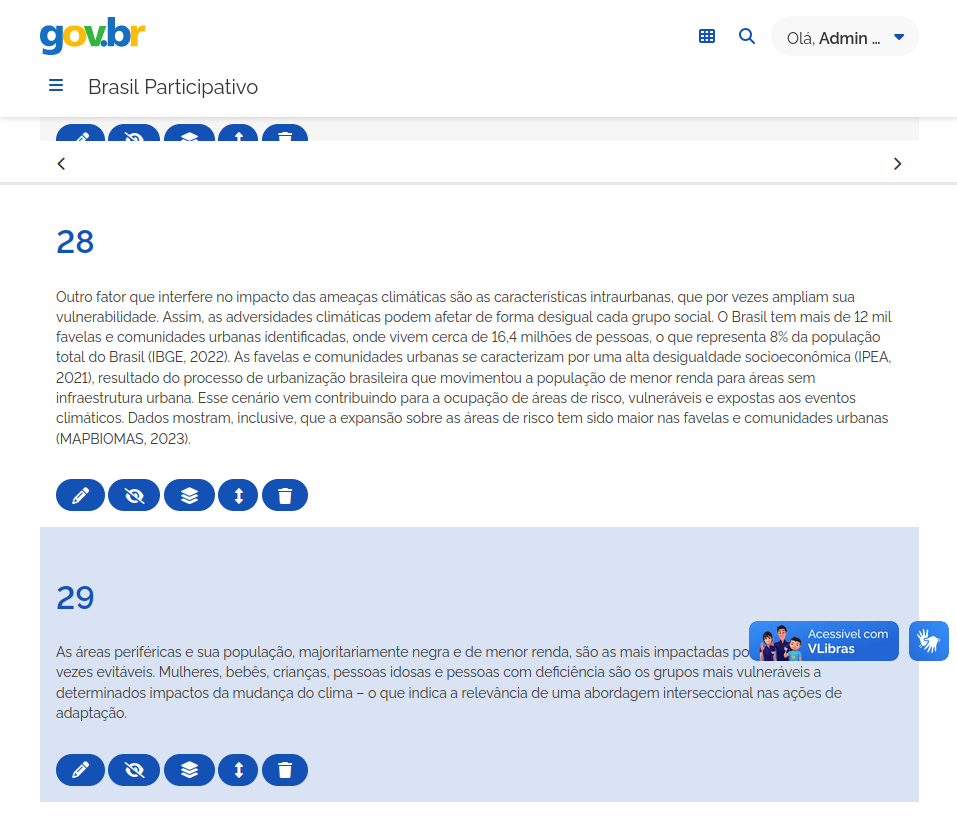
\includegraphics[width=\textwidth]{figuras/edicao-texto-v1.png}
  \fonte{Próprio autor}
\end{figure}

A página de edição conta com cinco ações possíveis:

\begin{itemize}
	\item Editar conteúdo do texto;
	\item Ocultar parágrafo;
	\item Mesclar parágrafos;
	\item Mover parágrafo;
	\item Remover parágrafo.
\end{itemize}

O \textit{Merge request} contendo as alterações descritas acima pode ser encontrado em \url{https://gitlab.com/lappis-unb/decidimbr/decidim-govbr/-/merge_requests/561}.

